\chapter{Results}
\section{t-test}
Nanopolish identified 21.5 million autosomal positions, thereof 20.5 million positions that passed the coverage filter and 8.8 million positions passed all quality controls. In Table \ref{table:signif_summary} the number of identified DMPs is shown for each thresholding method. These positions were then used to define the methylation profile of individuals with Kabuki syndrome.
\begin {table}
    \caption{Number of DMPs identified for each method}
    \begin{center}
        \begin{tabular}{p{5cm}p{5cm}} 
            \hline
             \textbf{Method} & \textbf{Number of DMP} \\
             \hline
             \hline
             \textbf{p-value} & 931,859 \\ 
             \textbf{p-value + $\Delta^*$} & 78,377 \\
             \textbf{Bonferroni} & 8,848,122\\ 
             \textbf{Bonferroni + $\Delta^*$} & 83,749 \\ 
             \textbf{Benjamini} & 23,717\\
             \textbf{Benjamini + $\Delta^*$} & 4,464 \\
             \hline            
             \multicolumn{2}{c}{             $^*$ $\Delta =$ where the difference between the average ratios exceeds 0.1} \\
        \end{tabular}
    \label{table:signif_summary}
    \end{center}
\end{table}

%Out of those 7 million, 4.3 million and 1 million positions were identified as DMPs based on significance level 0.05, 0.01 and  $1\cdot 10^{-6}$, respectively. After performing Bonferroni correction on the results that were significant given the 0.05 significance level, 154907 were significant. After calculating the adjusted p-values, 1.1 million positions were signifance given $\alpha = 0.05$.

% After removal of the sex chromosomes positions and extra chromosomes, high coverage regions and low coverage regions there were in total 20.5 million positions identified by Nanopolish.Out of those there were 2.1 million position significant given 0.05 significance threshold. 36 thousand positions were significant given the Bonferroni threshold, $2.44 \cdot 10^{-9}$. After calculating the adjusted p-values using the Benjamini-Hochberg procedure, assuming 25\% FDR, there were XXX positions significant, assuming 25\% FDR. 

\section{Fisher's exact test}
\label{section:results:Fisher-test}
We performed Fisher's exact test to see how well our results correlated with the results of Sobreira et al. \cite{sobreira2017patients}. These values were calculated without the quality control filter. The contingency tables and results are shown in Tables \ref{table:cont1}-\ref{table:cont5}. For Bonferroni treshold $=2.322 \times 10^{-9}$ we got p-value=$2\times 10^{-6}$ and OR=4.115, meaning that the odds of being in subset for significant sample (where subset refers to the set of DMPs identified by Sobreira et al.), is 4.12 times that for not significant. For all thresholds we got significantly higher odds of being significant if sample is in subset from Sobreira et al. \cite{sobreira2017patients} than not being in the subset, given 0.05 significant threshold.

% For Benjamini trehold of $\alpha=0.05$ we got p-value=$6 \times 10^{-6}$ and OR=2.244. For significance treshold=[0.05, 0.01, $10^{-6}$] we got p-value=[$3 \times 10^{-7}$, $10^{-8}$, $2\times 10^{-7}$] and OR=[1.545,1.704,2.381], respectively.

\begin {table}
    \centering
    \caption{Contingency tables}
    \begin{subtable}{1\linewidth}
        \centering
        \caption{For Bonferroni treshold, $\alpha = 2.322 \times 10^{-9}$}
            \begin{tabular}{c c c} 
                \hline
                &  \textbf{In subset} & \textbf{Not in subset} \\
                 \hline
                 \hline
                 \textbf{Significant} & 17 & 154,907 \\ 
                 \textbf{Not significant} & 570 & 21,373,454 \\
                 \hline
                 \multicolumn{3}{c}{p-value=$2\times 10^{-6}$, OR=4.115 } \\
                 \hline
            \end{tabular}
        \label{table:cont1}
    \end{subtable}
    ~\vspace*{1 cm}

    \begin{subtable}{1\linewidth}
        \centering
        \caption{For Benjamini-Hochberg treshold = $9.877\times10^{-3}$}
        \begin{tabular}{c c c} 
            \hline
            &  \textbf{In subset} & \textbf{Not in subset} \\
             \hline
             \hline
             \textbf{Significant} & 175 & 4,252,629 \\ 
             \textbf{Not significant} & 412 & 17,275,732 \\
             \hline
             \multicolumn{3}{c}{p-value=$4 \times 10^{-9}$, OR=1.726}\\
             \hline
        \end{tabular}
    \label{table:cont2}
    \end{subtable}
    ~\vspace*{1 cm}

    \begin{subtable}{1\linewidth}\
        \centering
        \caption{For 0.05 significance treshold}
        \begin{tabular}{c c c} 
            \hline
            &  \textbf{In subset} & \textbf{Not in subset} \\
             \hline
             \hline
             \textbf{Significant} & 249 & 6,951,183 \\ 
             \textbf{Not significant} & 338 & 14,577,178 \\
             \hline
             \multicolumn{3}{c}{p-value=$3 \times 10^{-7}$, OR=1.545}\\
             \hline
        \end{tabular}
    \label{table:cont3}
    \end{subtable}
    ~\vspace*{1 cm}

    \begin{subtable}{1\linewidth}
        \centering
        \caption{For 0.01 significance treshold}
        \begin{tabular}{c c c} 
            \hline
            &  \textbf{In subset} & \textbf{Not in subset} \\
             \hline
             \hline
             \textbf{Significant} & 174 & 4,267,808 \\ 
             \textbf{Not significant} & 413 & 17,260,553 \\
             \hline
            \multicolumn{3}{c}{p-value=$10^{-8}$, OR=1.704}\\
            \hline
        \end{tabular}
    \label{table:cont4}
    \end{subtable}
    ~\vspace*{1 cm}

     \begin{subtable}{1\linewidth}
        \centering
        \caption{Contingency table for $10^{-6}$ significance treshold}
         \begin{tabular}{c c c} 
            \hline
            &  \textbf{In subset} & \textbf{Not in subset} \\
             \hline
             \hline
             \textbf{Significant} & 49 & 793,010 \\ 
             \textbf{Not significant} & 538 & 20,735,351 \\
             \hline
            \multicolumn{3}{c}{p-value=$2\times 10^{-7}$, OR=2.381}\\
            \hline
        \end{tabular}
    \label{table:cont5}
     \end{subtable}
\end{table}

%Out of those position 2.2 million, 872 thousand and 22 thousand position were identified within genes and additionally 552, 199 and 5 positions within 5 bases from genes, for each significance level respectively.

%Of the ones that occurred within genes, there were multiple genes that had many occurences, including ESR1, TSPAN4, GARS, MYO1F, SOX18, AGAP2 and TJP1 as mentioned in the Sobreira et. al (2017) paper \cite{sobreira2017patients}. However the most common genes included ... !!! 
%%%%%%%%%%%%%%% WHICH ONES TO MENTION?!
% Of those: significant from 0.05 all + TJP1
% 0.01: All + TJP1
% 10e-6: ESR1, GARS, MYO1F, SOX18, TJP1


\section{PCA}
\label{section:results:PCA}
\subsection{1 million random features}
The results for the PCA using 1 million random features are shown in Figure \ref{fig:1m-pca}. We can see that there is no obvious clustering of the two groups and each PC explains small percentage of the variance, as seen in Figure \ref{fig:1m-varexpl}. In the other three plots (PC3 vs PC4, PC5 vs PC6, PC7 vs PC8) we can see that there are outliers in the Kabuki group. Many of the Kabuki samples do not have high enough coverage, causing a lot of nan values to be introduced. Since we perform mean imputation, the low coverage Kabuki samples tend to cluster with the normal group, where the mean lies. 

\FloatBarrier
\begin{figure}[!h]
    \centering
    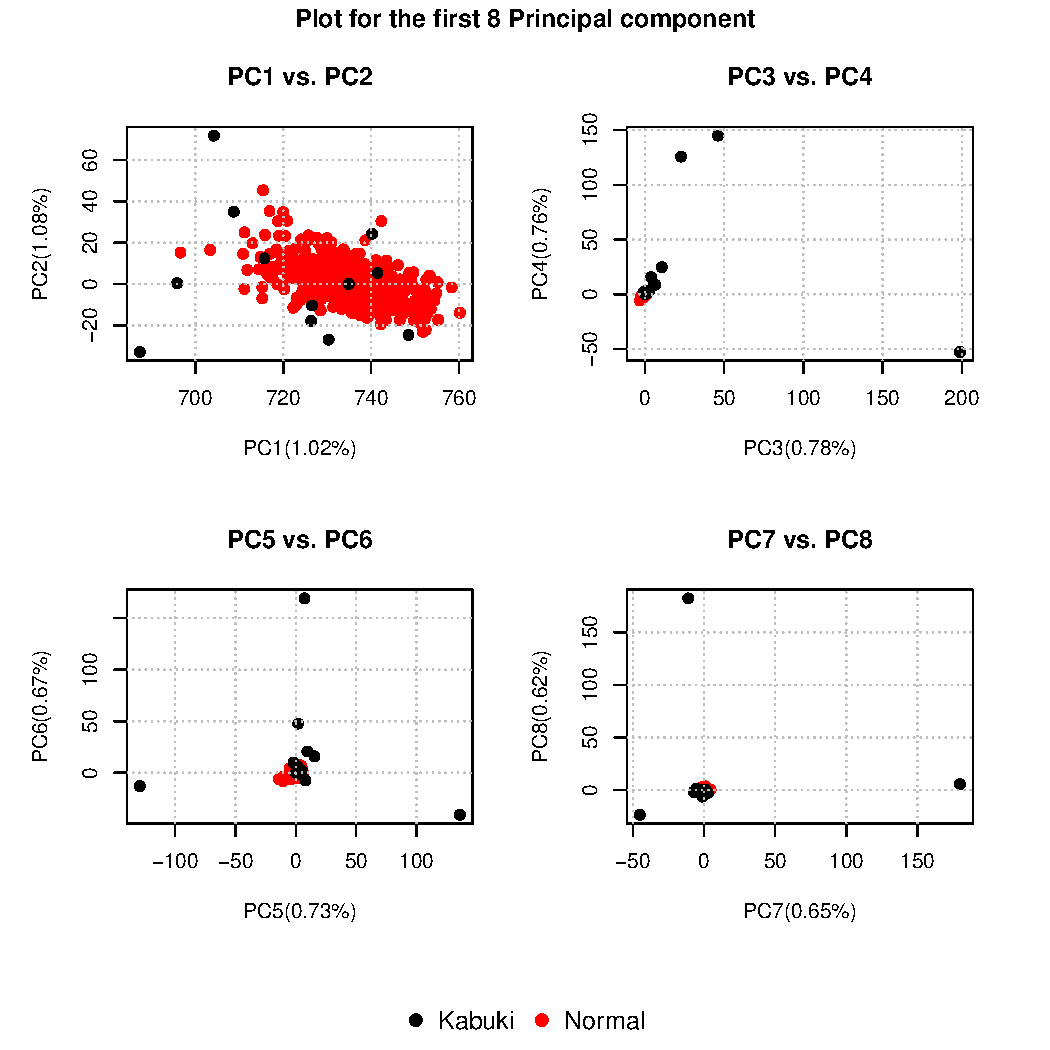
\includegraphics[width=\textwidth]{figures/PCA/1m/pca_plot.pdf}
    \caption{PCA plot for 1 million random features}
    \label{fig:1m-PCA}
\end{figure}

\begin{figure}[!h]
    \centering
    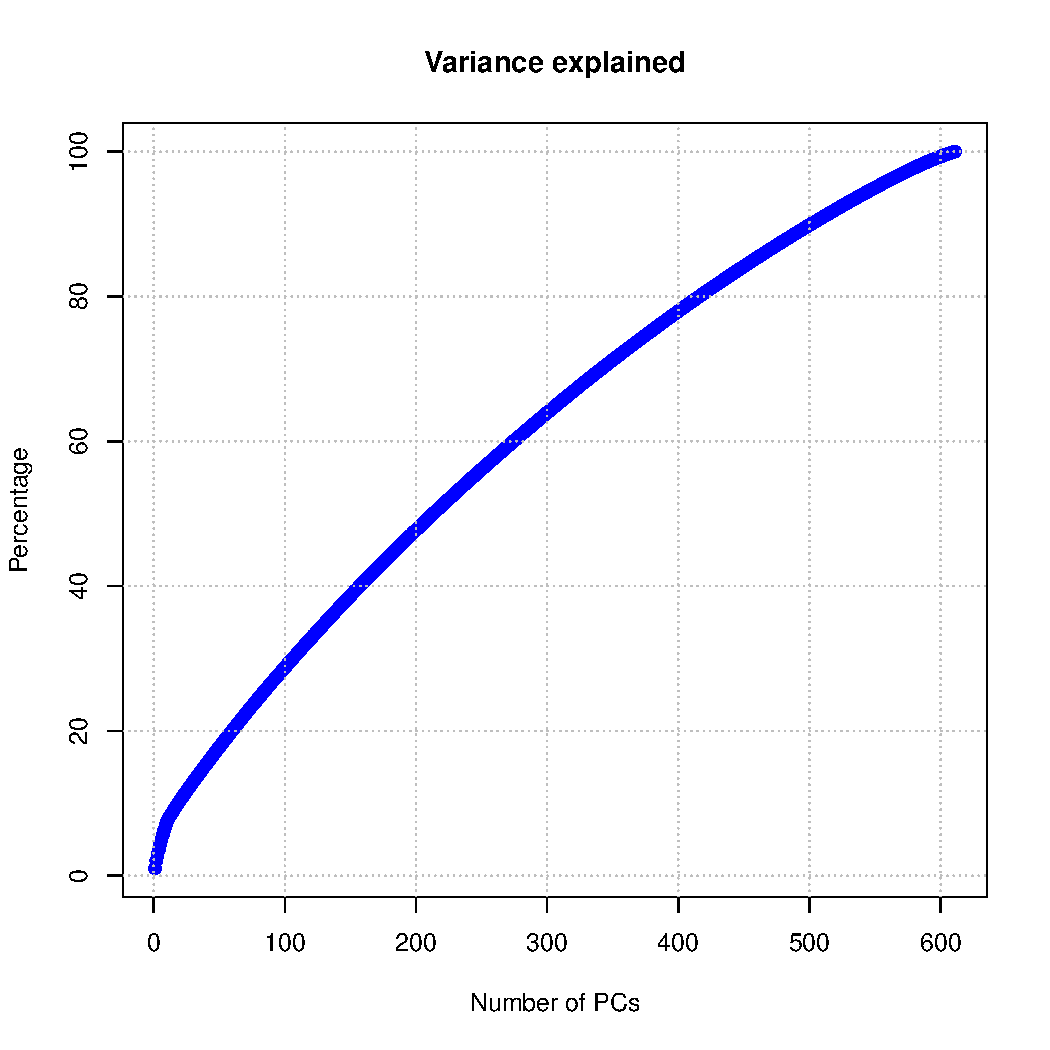
\includegraphics[width=0.5\columnwidth]{figures/PCA/1m/var_expl.pdf}
    \caption{Variance explained plot for 1 million random features}
    \label{fig:1m-varexpl}
\end{figure}
\FloatBarrier

\subsection{590 features}
In the first subplot in Figure \ref{fig:590-PCA} we can see that we can separate the groups using linear classifier, which indicates that those positions indeed are relevant for the Kabuki syndrome.

\begin{figure}[!h]
    \centering
    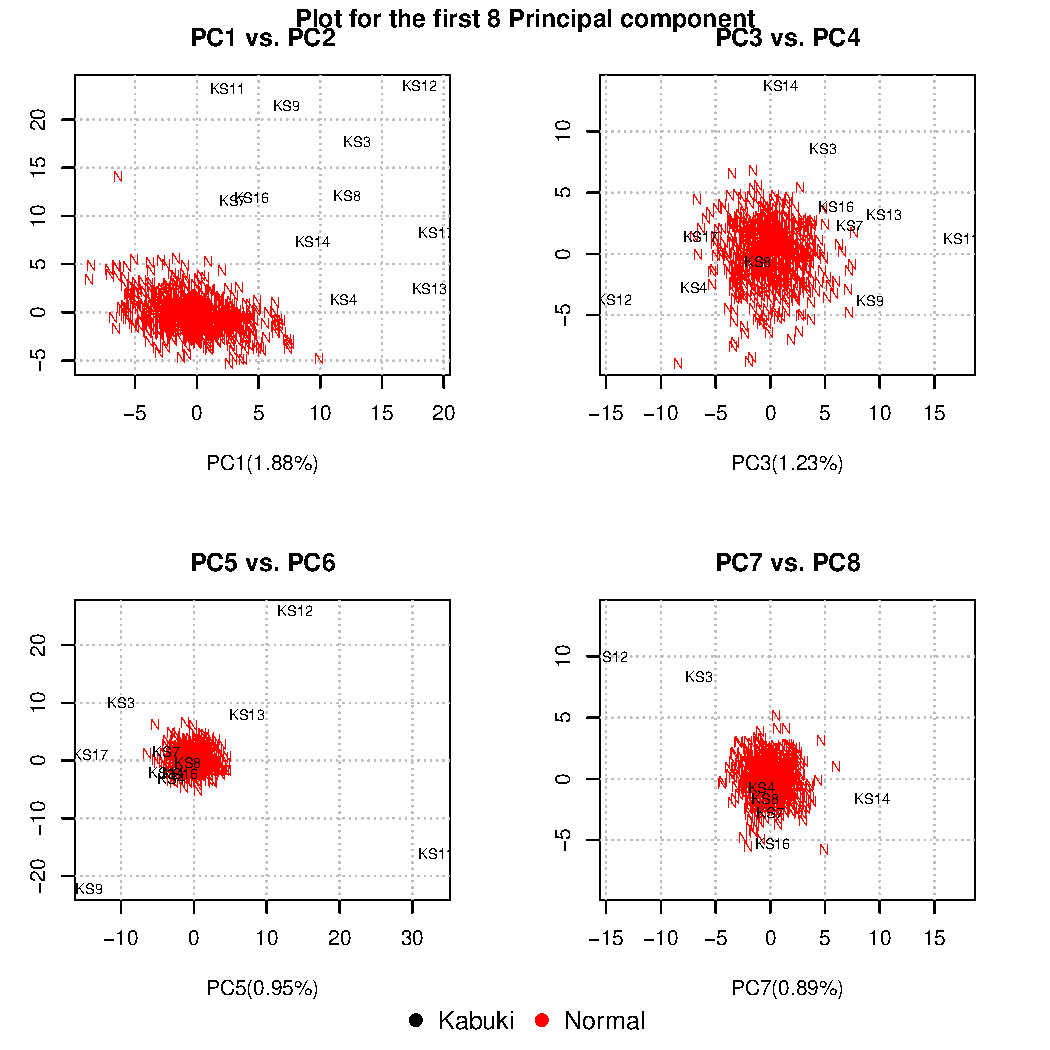
\includegraphics[width=\textwidth]{figures/PCA/590/pca_plot_label.pdf}
    \caption{PCA plot for 590 features known to be related to Kabuki syndrome}
    \label{fig:590-PCA}
\end{figure}
\begin{figure}[!h]
    \centering
    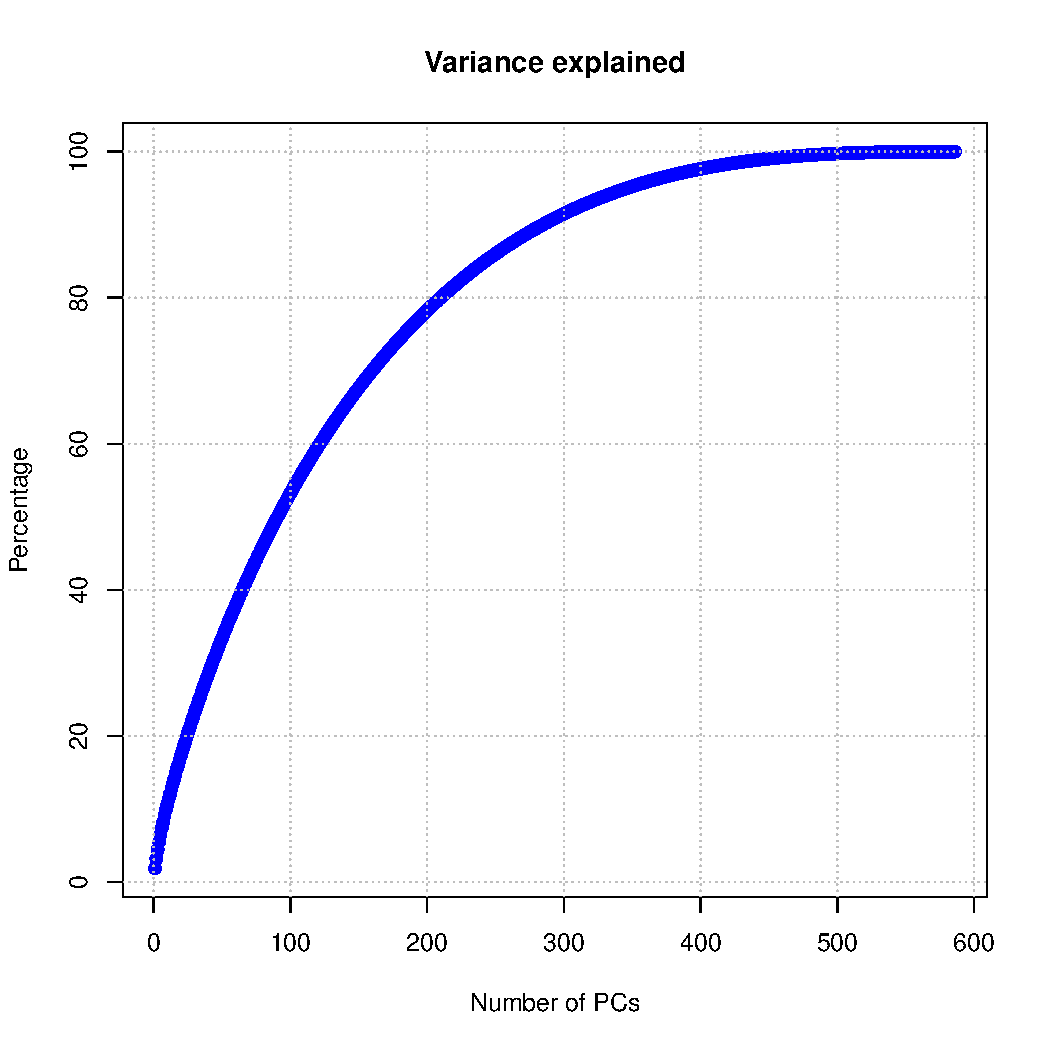
\includegraphics[width=0.5\columnwidth]{figures/PCA/590/var_expl.pdf}
    \caption{Variance explained plot for 590 features known to be related to Kabuki syndrome}
    \label{fig:590-varexpl}
\end{figure}
\

\subsection{Age matched dataset}
We performed PCA on all features (~22 million) of the age matched dataset. In Figure \ref{fig:case_control}-\ref{fig:case_control-sex} similarly as before we can see a lot more outliers in the Kabuki group. In the third subplot (PC5 vs PC6) we can almost perfectly separate the two groups using vertical line, however the other plots do not show decisive clustering.
\
\begin{figure}[!h]
    \centering
    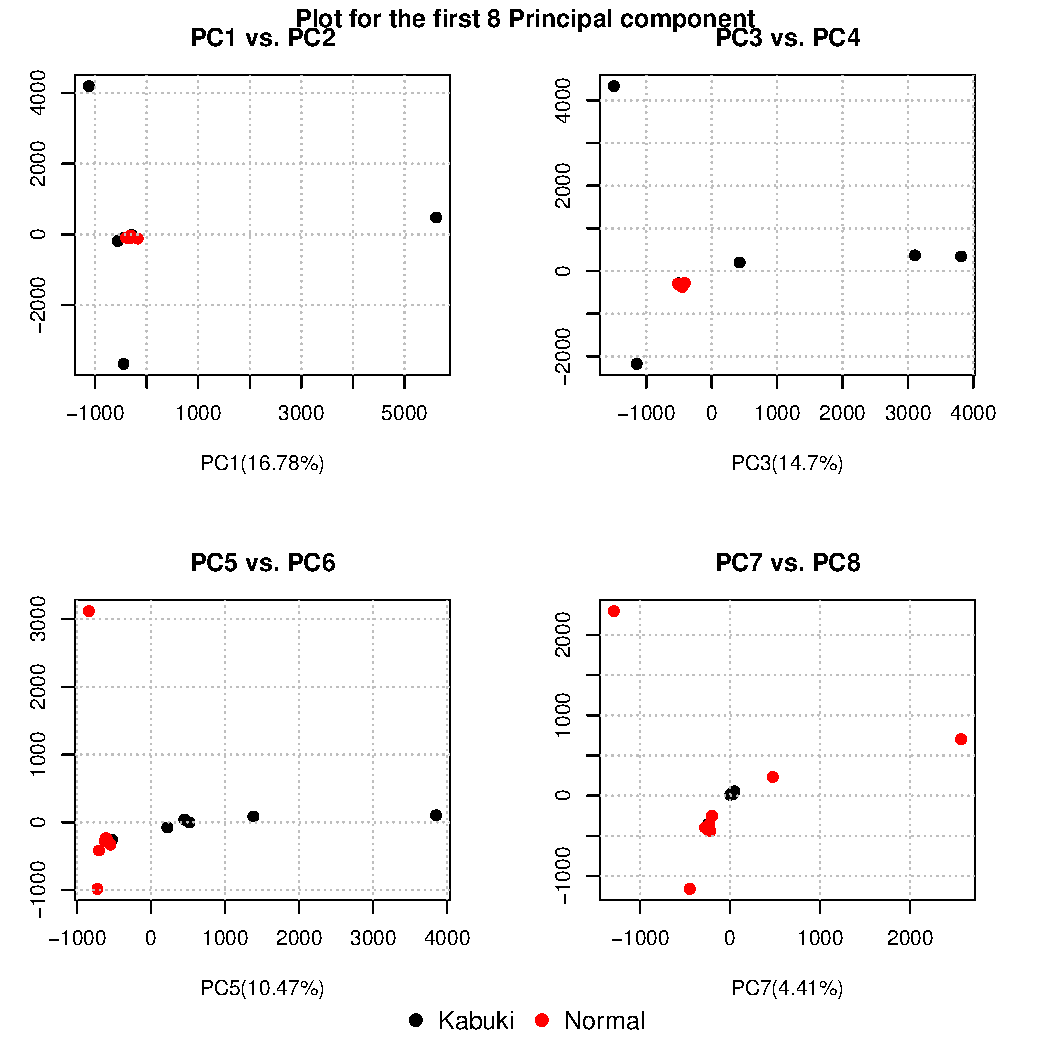
\includegraphics[width=\textwidth]{figures/PCA/case_control/pca_plot.pdf}
    \caption{PCA for the age matched dataset}
    \label{fig:case_control}
\end{figure}

\begin{figure}[!h]
    \centering
    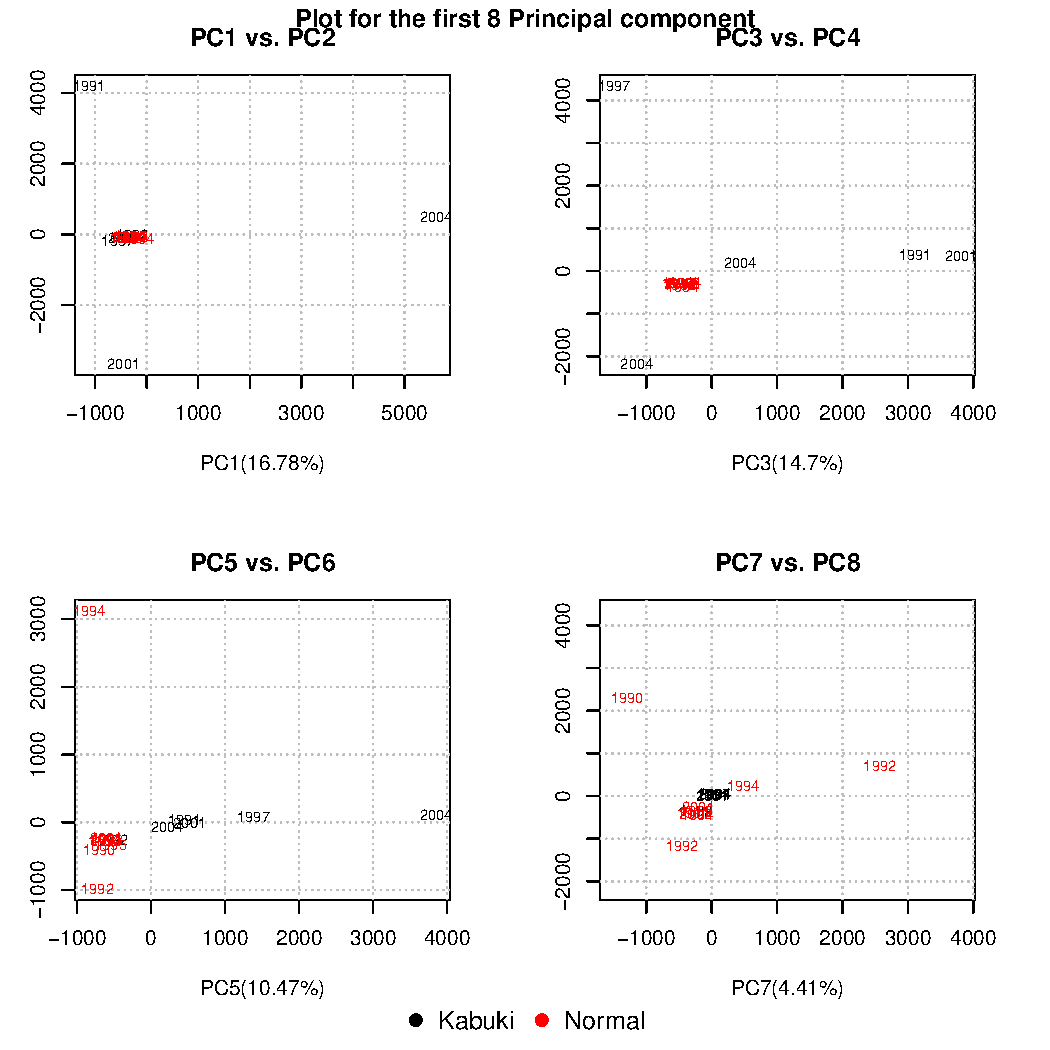
\includegraphics[width=\textwidth]{figures/PCA/case_control/age_PCA.pdf}
    \caption{PCA for the age matched dataset, with birth year displayed on the graph}
    \label{fig:case_control-age}
\end{figure}

\begin{figure}[!h]
    \centering
    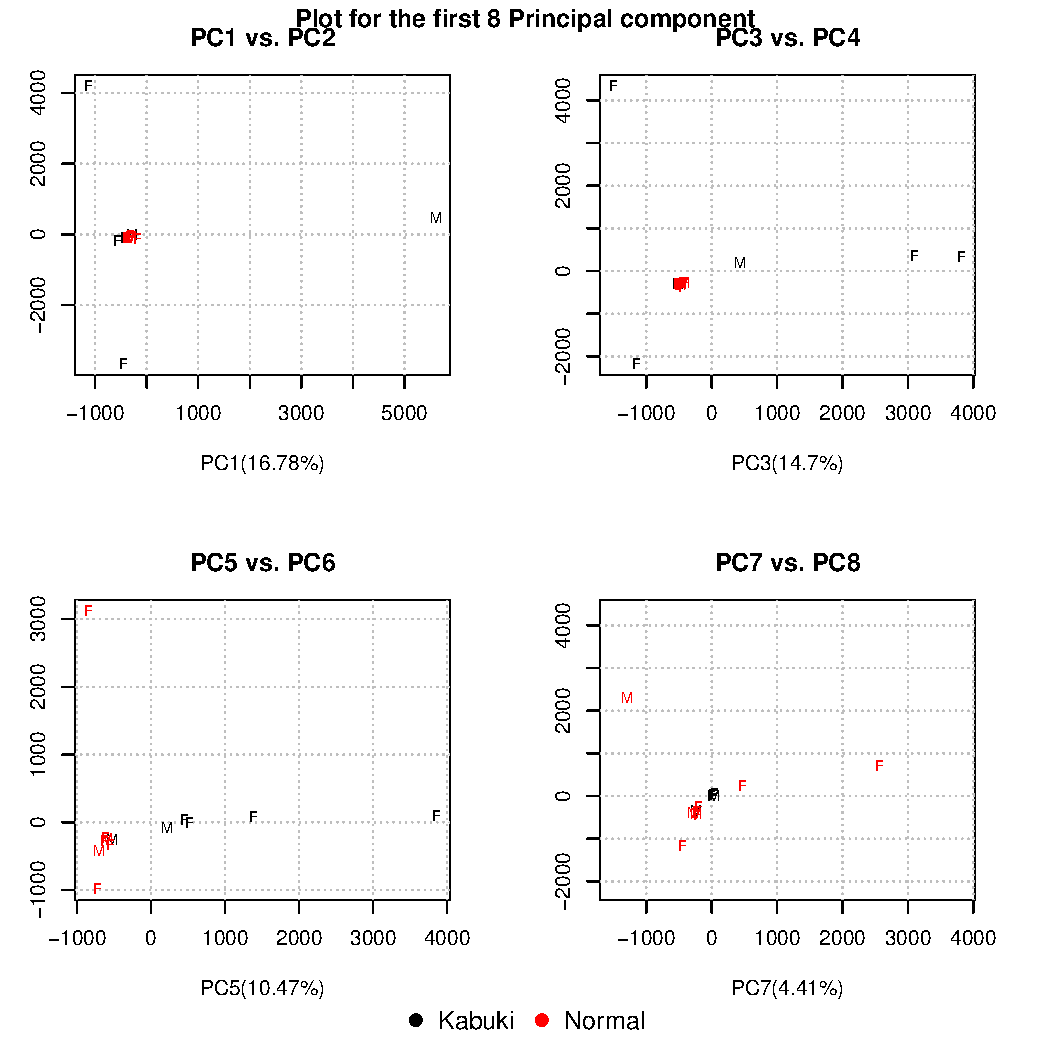
\includegraphics[width=\textwidth]{figures/PCA/case_control/sex_PCA.pdf}
    \caption{PCA for the age matched dataset, with sex displayed on the graph}
    \label{fig:case_control-sex}
\end{figure}




\subsection{Kabuki divided in two age groups}
We performed PCA on all features (~22 million) in the dataset. In Figure \ref{fig:oldyoung-pca} we have no clear clustering.
\begin{figure}[!h]
    \centering
    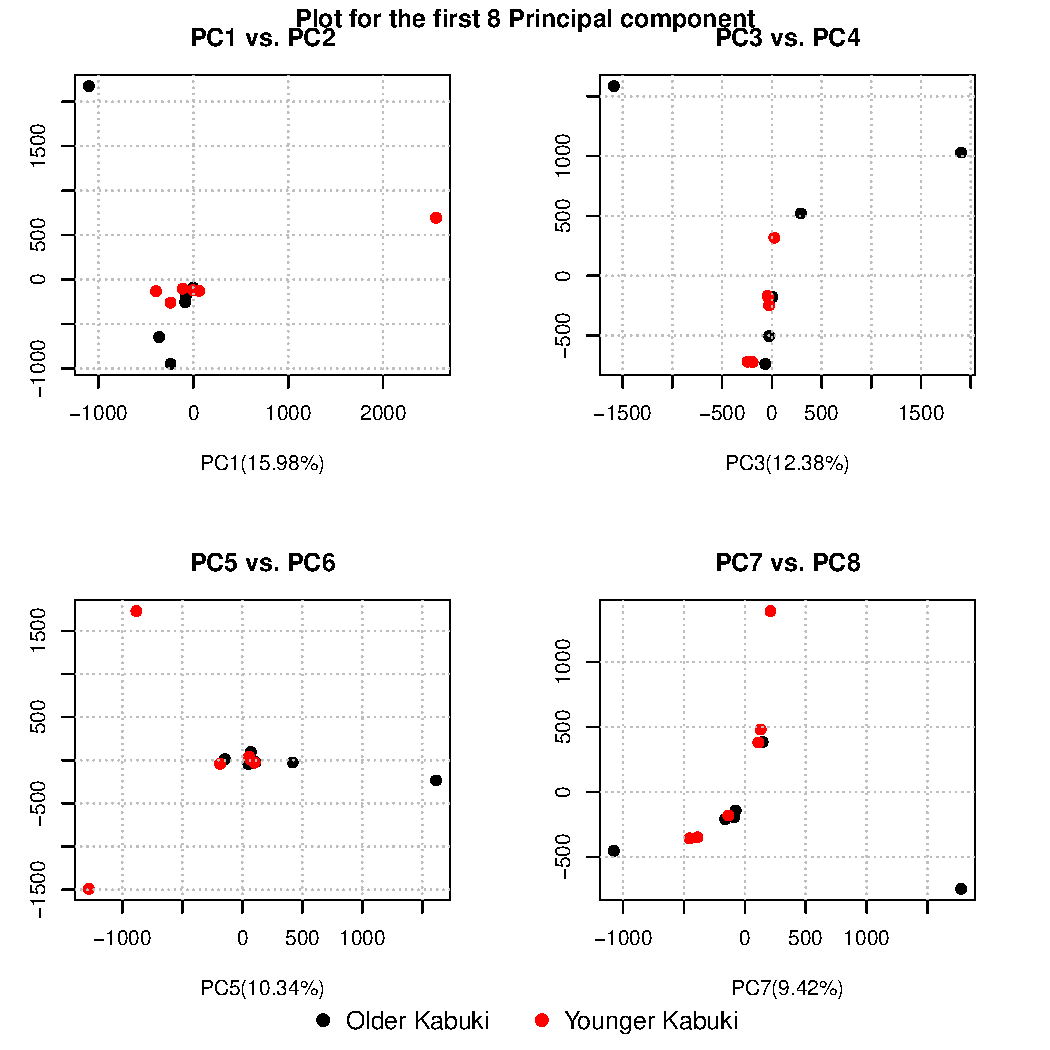
\includegraphics[width=\textwidth]{figures/PCA/old_young/pca_plot.pdf}
    \caption{PCA for the age divided kabuki dataset}
    \label{fig:oldyoung-pca}
\end{figure}
%%%%%%%%%%%%%%%%%%%%%%%%%%%%%%%%%%%%%%%%%%%%%%%%%%%%%%%%%%%%%%%%%%%%%%%%%%%%%%%%%%%
\iffalse
\begin{figure}[!h]
    \centering
    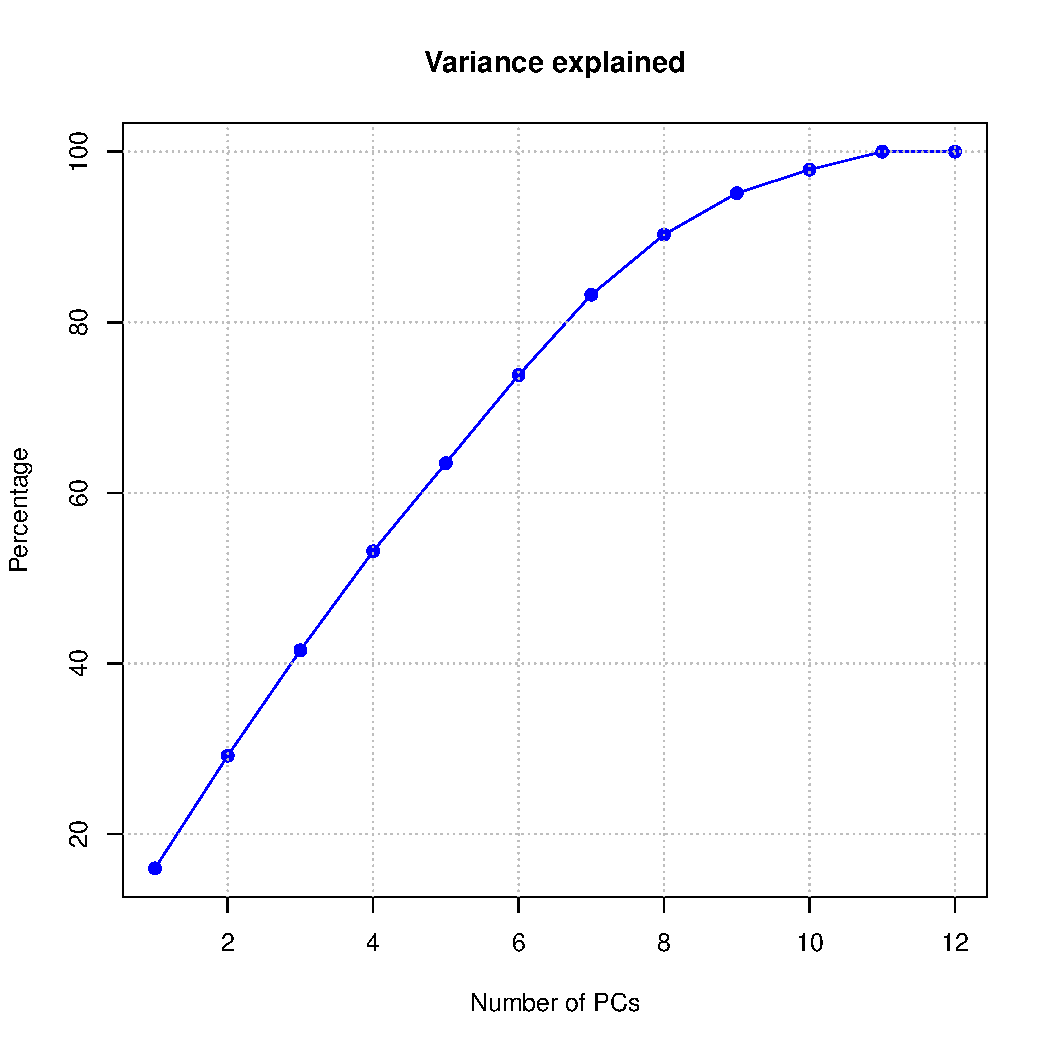
\includegraphics[width=0.6\columnwidth]{figures/PCA/old_young/var_expl.pdf}
    \caption{Variance explained for the age divided kabuki dataset}
    \label{fig:oldyoung-varexpl}
\end{figure}
\fi
%%%%%%%%%%%%%%%%%%%%%%%%%%%%%%%%%%%%%%%%%%%%%%%%%%%%%%%%%%%%%%%%%%%%%%%%%%%%%%%%%%


\subsection{Called with certainty}

\begin{figure}[!h]
    \centering
    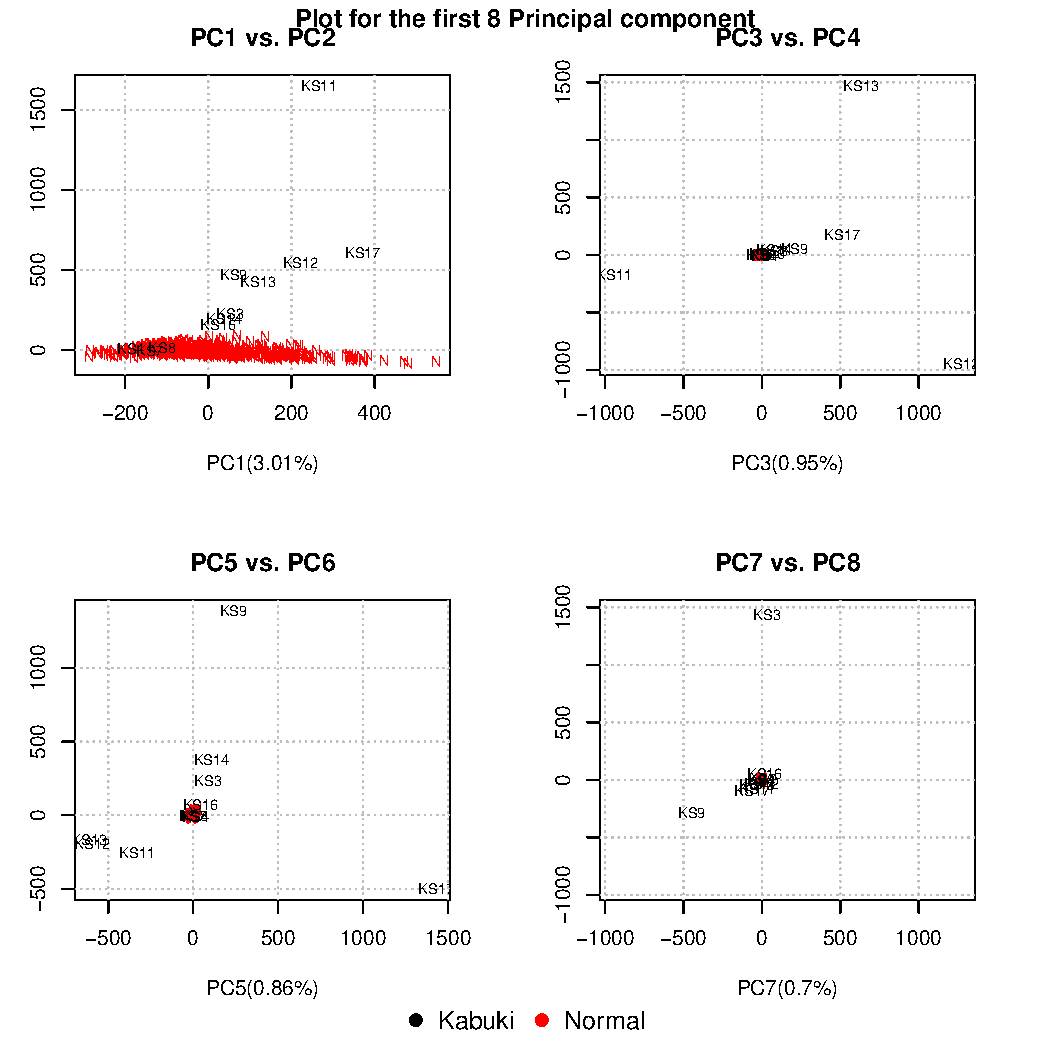
\includegraphics[width=\textwidth]{figures/PCA/certain/pca_plot_label.pdf}
    \caption{PCA plot for the features where nanopolish called methylation or non-methylation in over 90\% of the reads}
    \label{fig:certain-PCA}
\end{figure}

%%%%%%%%%%%%%%%%%%%%%%%%%%%%%%%%%%%%%%%%%%%%%%%%%%%%%%%%%%%%%%%%%%%%%%%%%%%%%%%%%%%
\iffalse
\begin{figure}[!h]
    \centering
    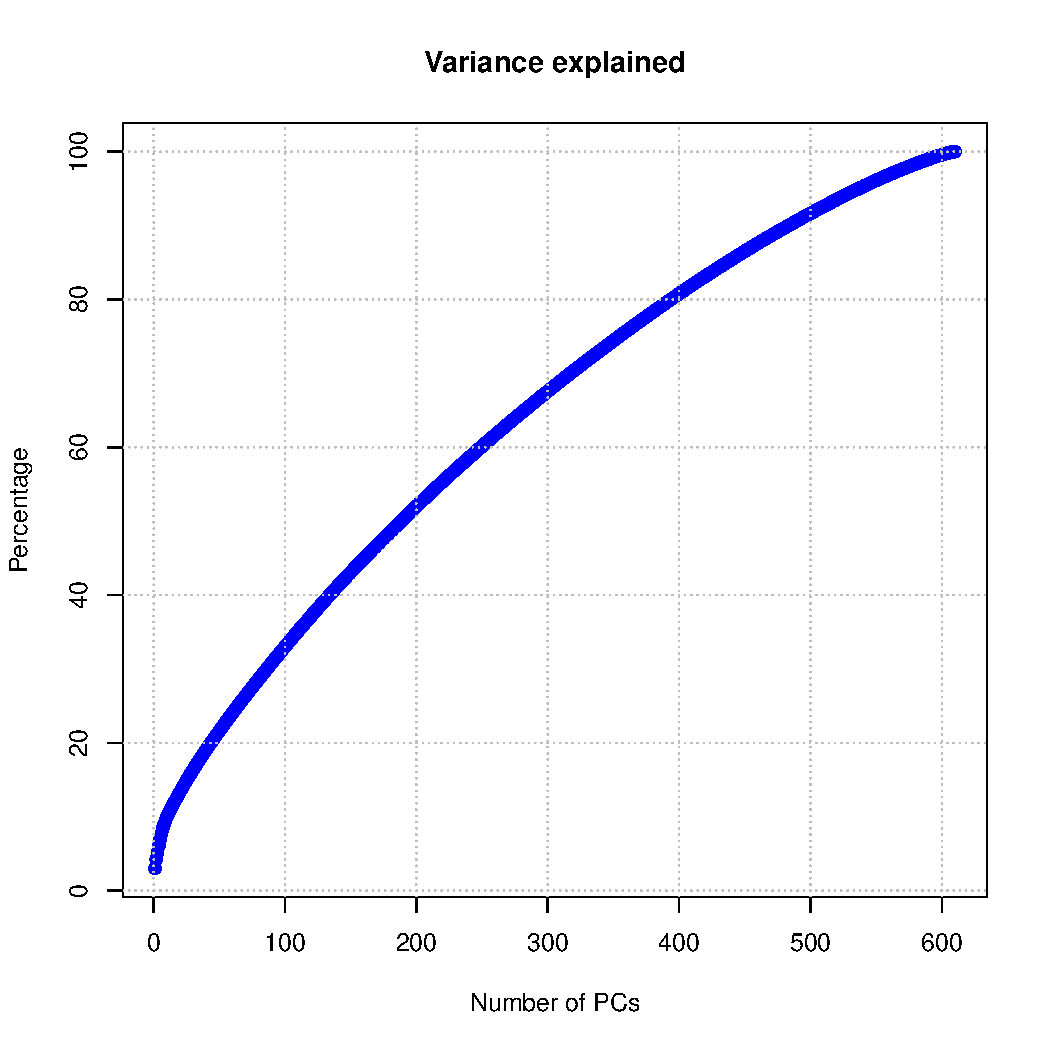
\includegraphics[width=0.6\columnwidth]{figures/PCA/certain/var_expl.pdf}
    \caption{Variance explained plot for the features where nanopolish called methylation or non-methylation in over 90\% of the reads}
    \label{fig:certain-varexpl}
\end{figure}
\fi
%%%%%%%%%%%%%%%%%%%%%%%%%%%%%%%%%%%%%%%%%%%%%%%%%%%%%%%%%%%%%%%%%%%%%%%%%%%%%%%%%%

\subsubsection{Bivalent regions}
\begin{figure}[!h]
    \centering
    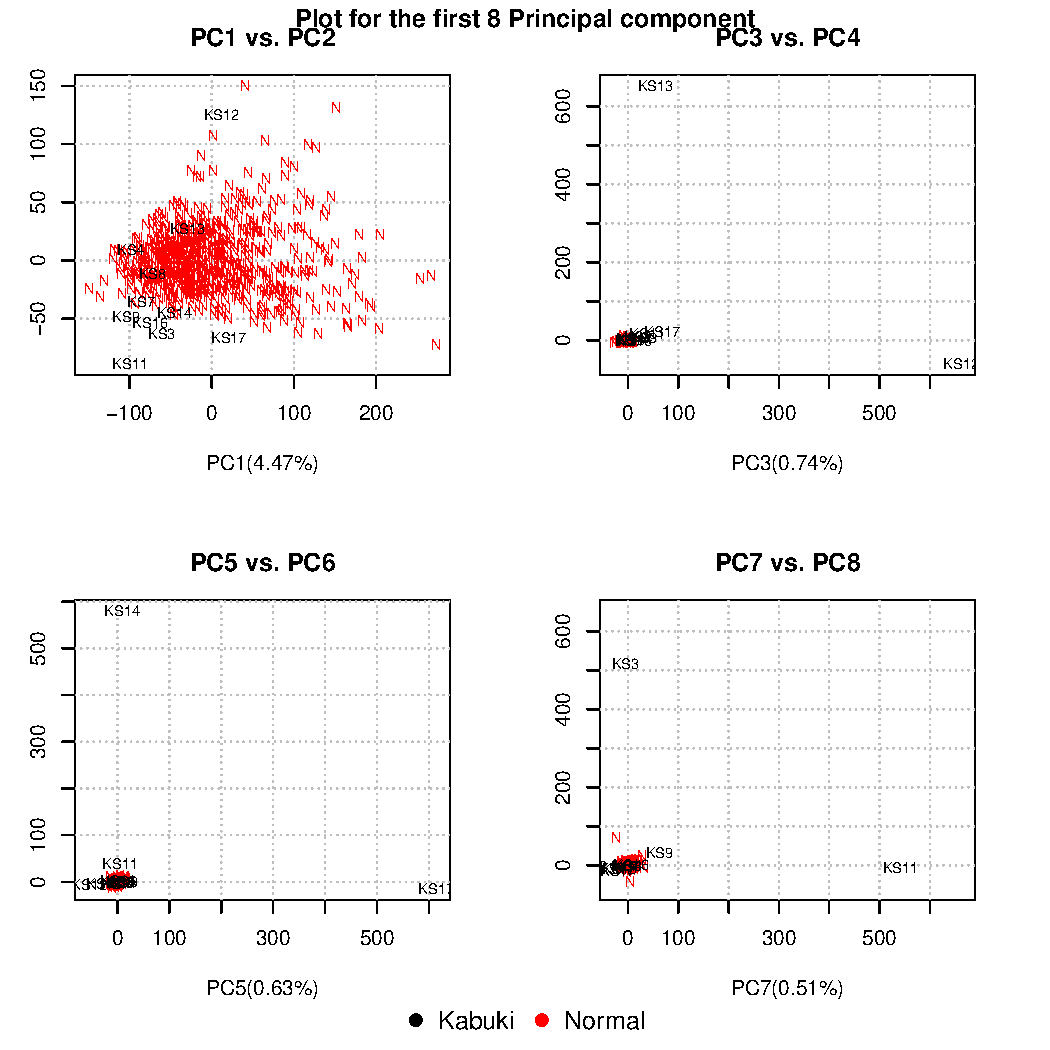
\includegraphics[width=\textwidth]{figures/PCA/bivalent/pca_plot_label.pdf}
    \caption{PCA plot for the features where nanopolish called methylation or non-methylation in over 90\% of the reads, within bivalent regions}
    \label{fig:bivalent-PCA}
\end{figure}

%%%%%%%%%%%%%%%%%%%%%%%%%%%%%%%%%%%%%%%%%%%%%%%%%%%%%%%%%%%%%%%%%%%%%%%%%%%%%%%%%%%
\iffalse
\begin{figure}[!h]
    \centering
    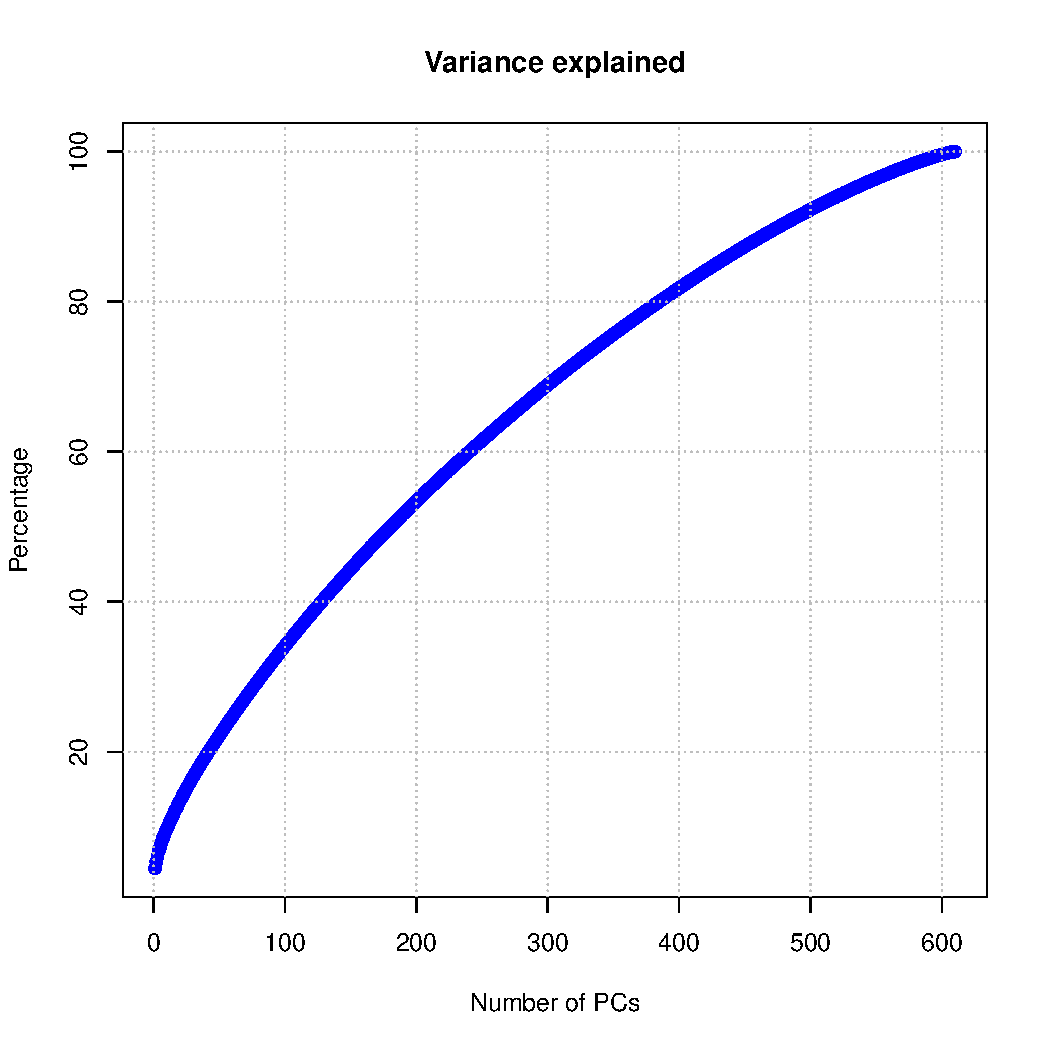
\includegraphics[width=0.6\columnwidth]{figures/PCA/bivalent/var_expl.pdf}
    \caption{Variance explained plot for the features where nanopolish called methylation or non-methylation in over 90\% of the reads, within bivalent regions}
    \label{fig:bivalent-varexpl}
\end{figure}
\fi
%%%%%%%%%%%%%%%%%%%%%%%%%%%%%%%%%%%%%%%%%%%%%%%%%%%%%%%%%%%%%%%%%%%%%%%%%%%%%%%%

\subsection{Consistency between plus and minus strand}

\begin{figure}[!h]
    \centering
    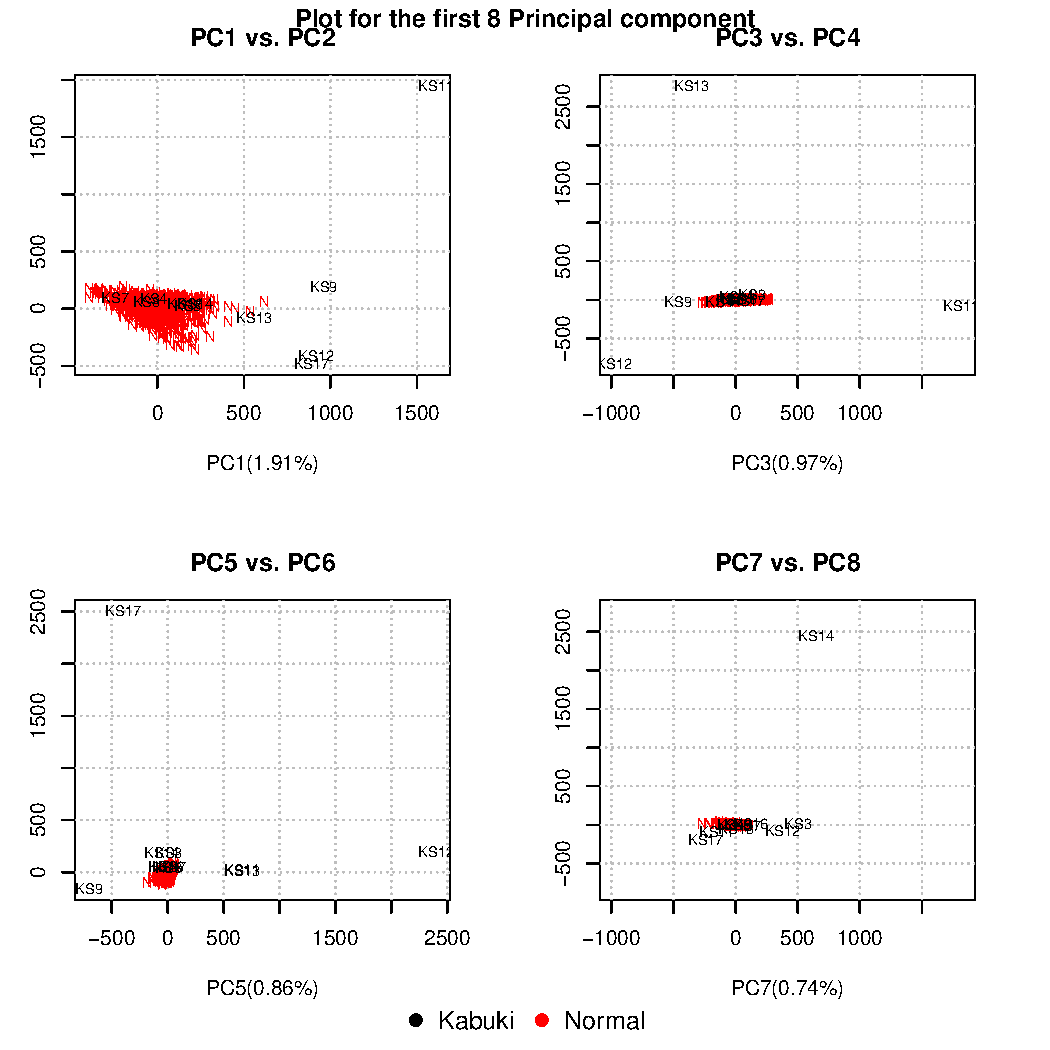
\includegraphics[width=\textwidth]{figures/PCA/plus_minus/pca_plot_label.pdf}
    \caption{PCA plot for the features where nanopolish had less than 0.5\% difference between the plus strand and minus strand}
    \label{fig:certain-PCA}
\end{figure}

%%%%%%%%%%%%%%%%%%%%%%%%%%%%%%%%%%%%%%%%%%%%%%%%%%%%%%%%%%%%%%%%%%%%%%%%%%%%%%%%%%%
\iffalse
\begin{figure}[!h]
    \centering
    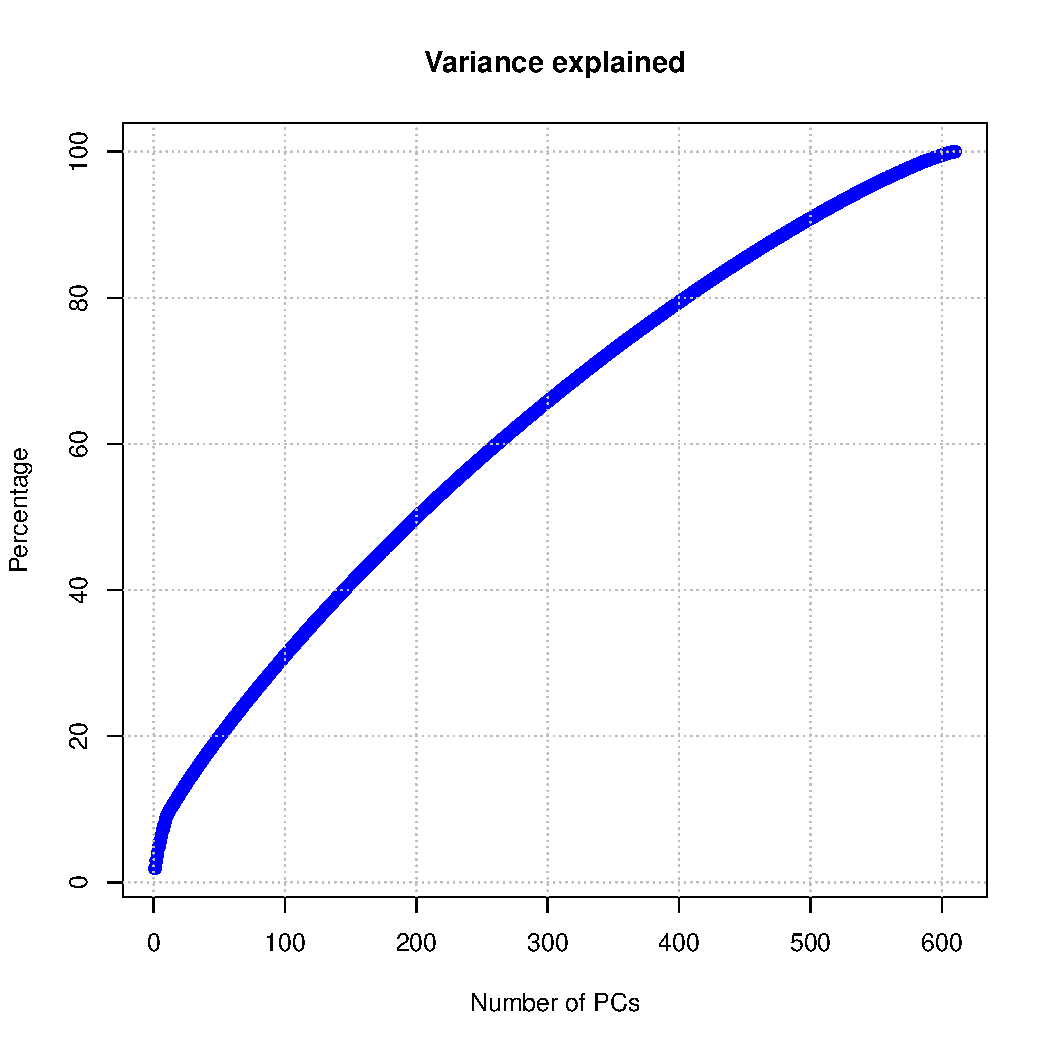
\includegraphics[width=0.6\columnwidth]{figures/PCA/plus_minus/var_expl.pdf}
    \caption{Variance explained plot for the features where nanopolish had less than 0.5\% difference between the plus strand and minus strand}
    \label{fig:certain-varexpl}
\end{figure}
\fi
%%%%%%%%%%%%%%%%%%%%%%%%%%%%%%%%%%%%%%%%%%%%%%%%%%%%%%%%%%%%%%%%%%%%%%%%%%%%%%%%%

\subsection{590 larger}
\iffalse
\begin{figure}[!h]
    \centering
    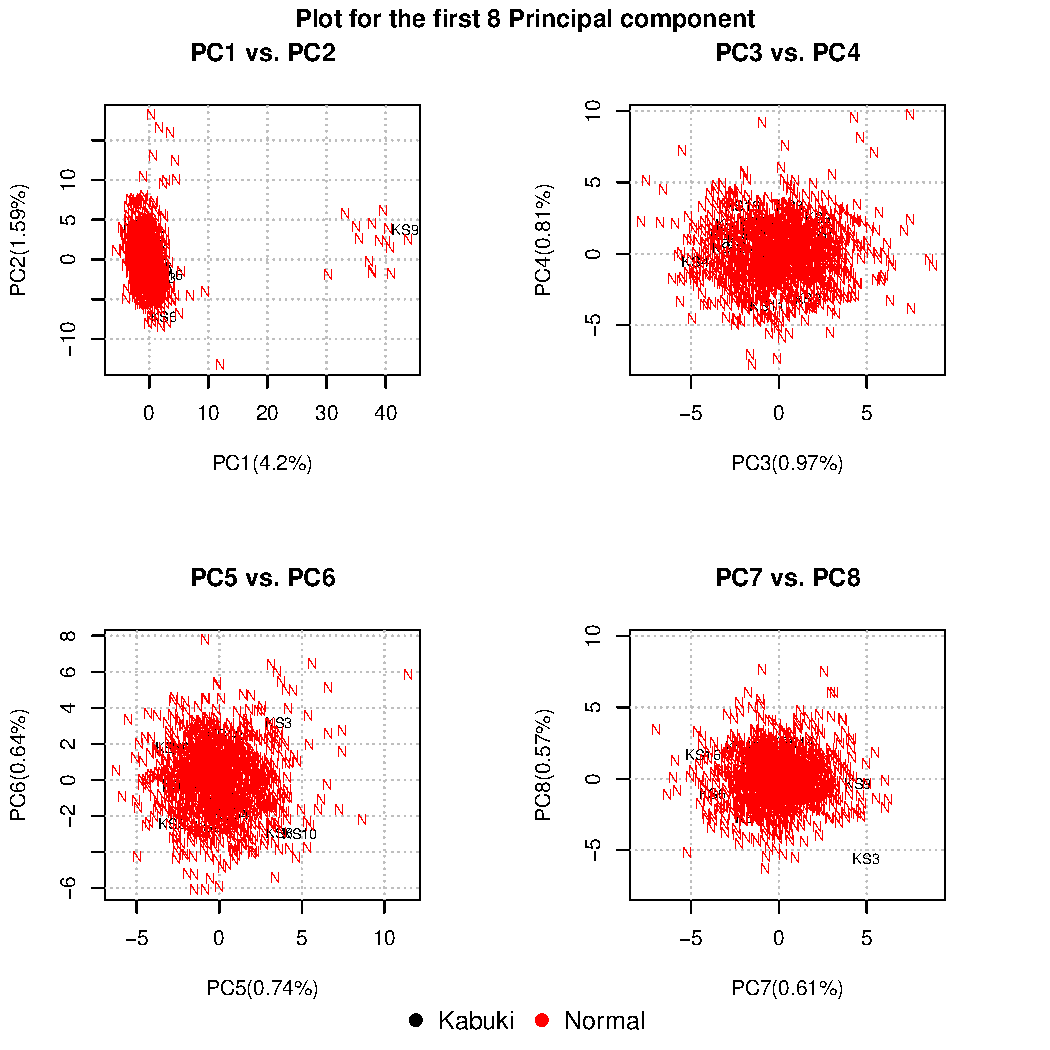
\includegraphics[width=\textwidth]{figures/PCA/590/pca_plot_label_larger.pdf}
    \caption{PCA plot for the final dataset, for the 590 positions identified by H.Tomasson.}
    \label{fig:certain-PCA}
\end{figure}

\subsection{Certain larger}

\begin{figure}[!h]
    \centering
    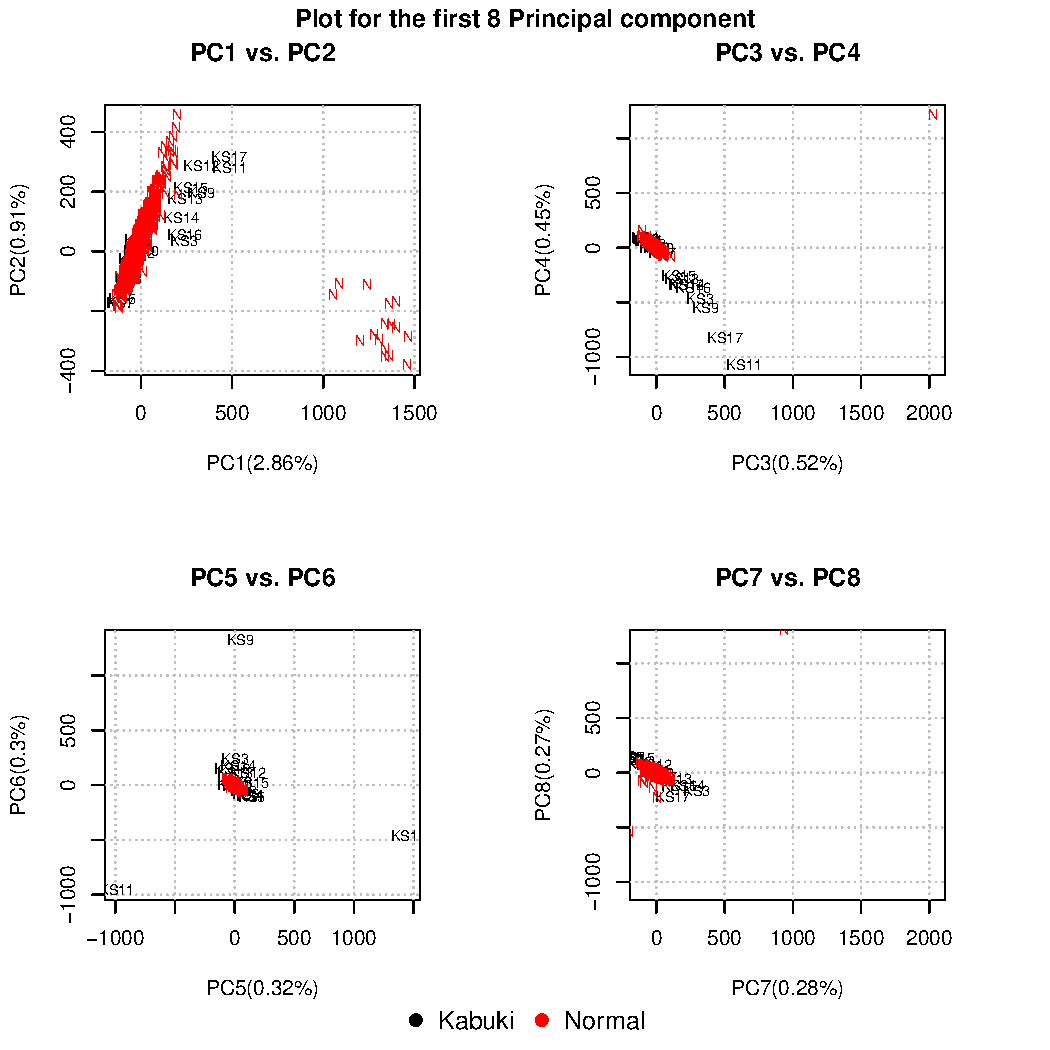
\includegraphics[width=\textwidth]{figures/PCA/certain/pca_plot_label_larger.pdf}
    \caption{PCA plot for the final dataset, where methylation or non-methylation was called in >75\% of the reads..}
    \label{fig:certain-PCA}
\end{figure}
\fi 

\subsection{Bonferroni}
\begin{figure}[!h]
    \centering
    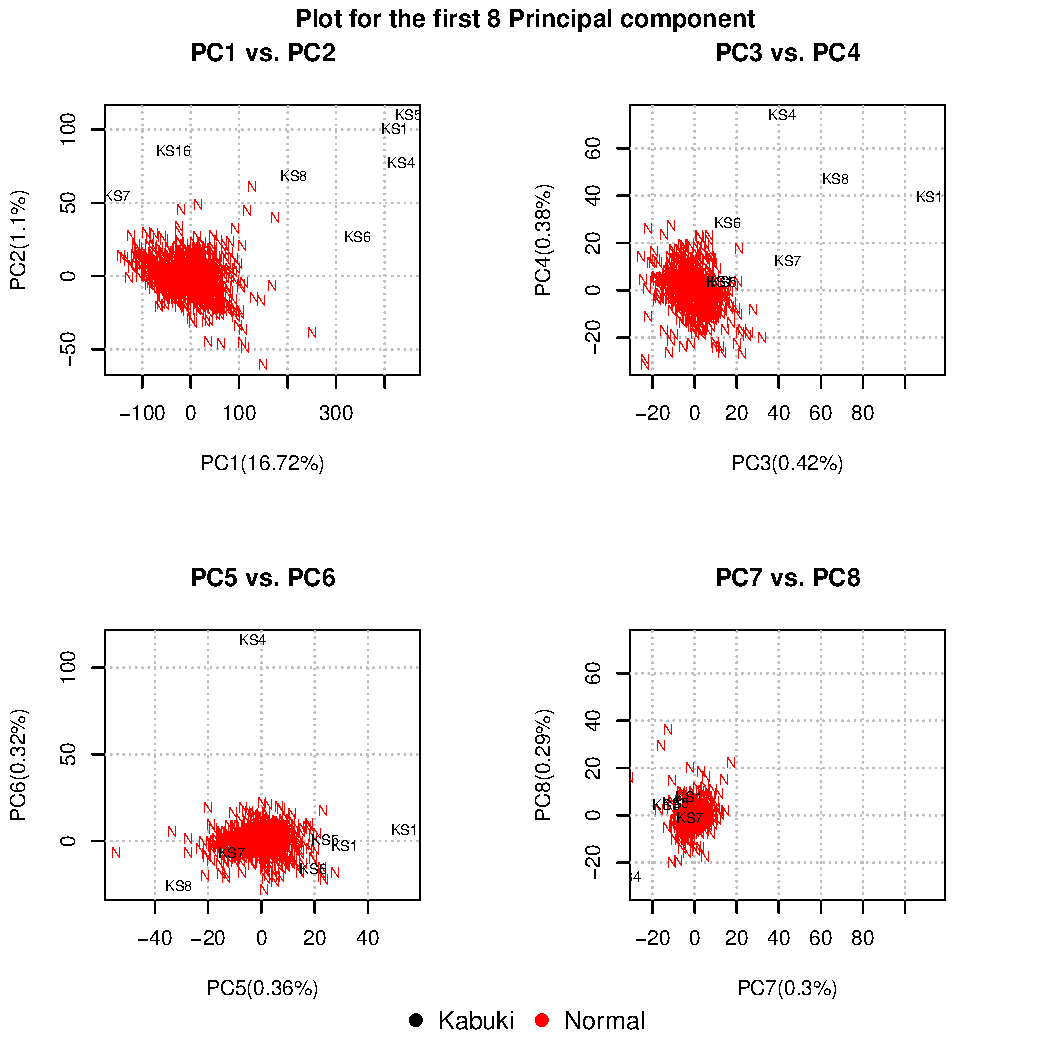
\includegraphics[width=\textwidth]{figures/PCA/bonferroni/pca_plot_label.pdf}
    \caption{PCA plot are considered significantly differentially methylated given the bonferroni threshold}
    \label{fig:bonferroni-PCA}
\end{figure}


\section{Hierarchical clustering}
We performed Hierarchical clustering using dist() and hclust() in R \ref{fig:hclust}. It can be seen that most of the Kabuki samples form a cluster, however there are three kabuki samples distributed within the control group.

\begin{figure}[!h]
    \begin{centering}
    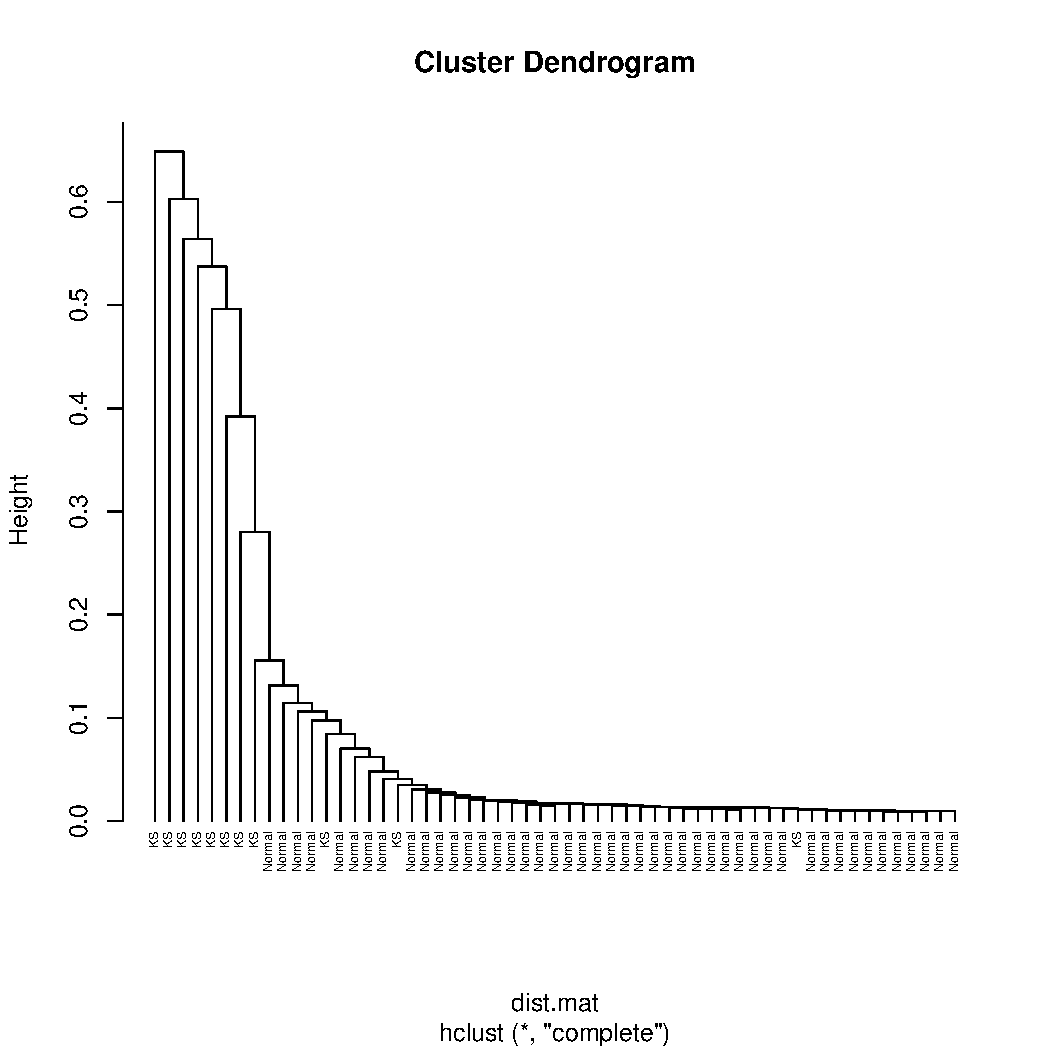
\includegraphics[width=0.7\columnwidth]{figures/hclust.pdf} 
    \caption[Hierachical clustering]{\textbf{Hierarchical clustering.} Clustering bla bla bla}    
    \label{fig:hclust}
    \end{centering}
\end{figure}

% Also insert from the 590

\section{Average methylation per grop}

\begin{figure}[!h]
    \begin{centering}
    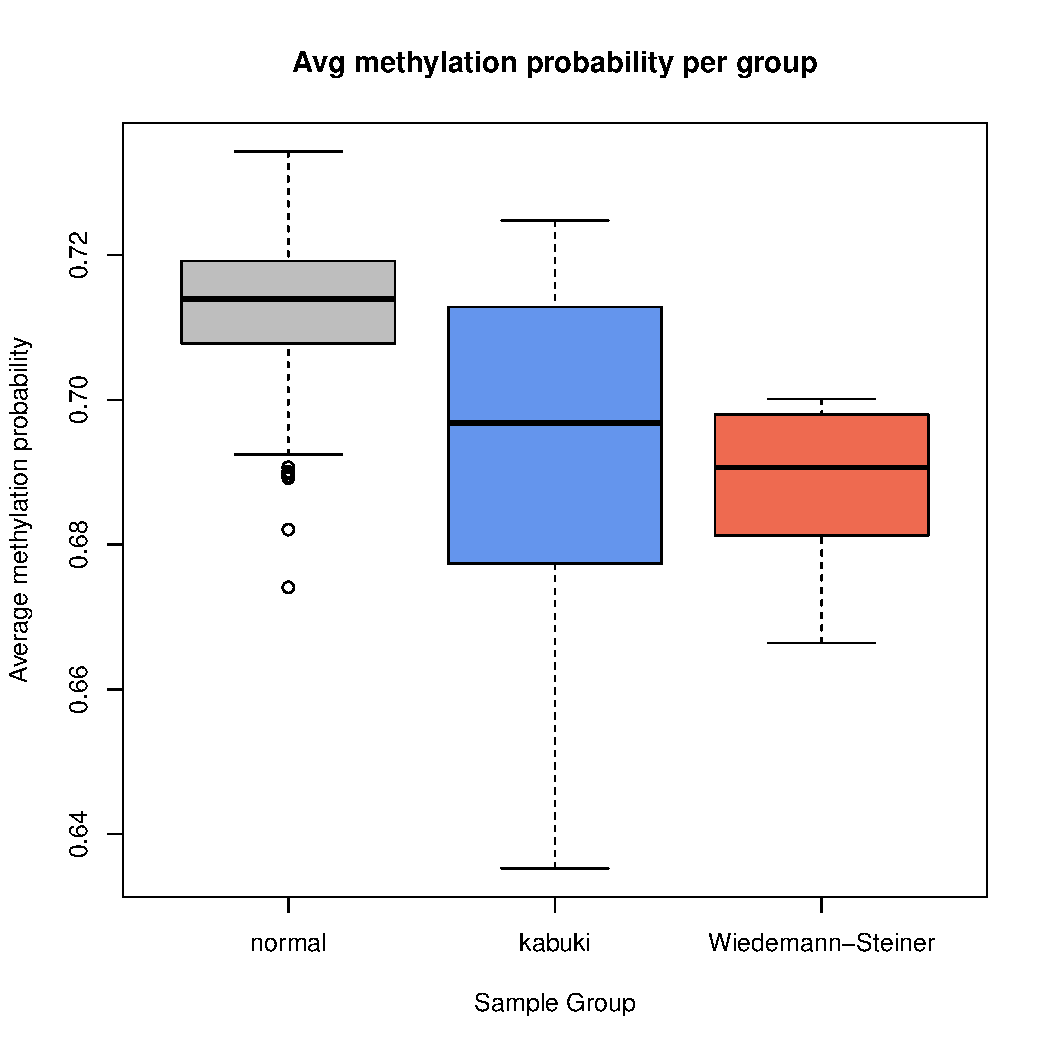
\includegraphics[width=0.7\columnwidth]{figures/avg_met_per_group.pdf} 
    \caption[Average methylation per sample group]{\textbf{Average methylation per group.} We can see that the average methylation for the normal group is a little bit higher then for the other two. However we also have more samples and therefore the measurement is also more accurate.}    
    \label{fig:hclust}
    \end{centering}
\end{figure}

\section{Nanopolish performance}
\label{section:results:Nanopolish-performance}
We took the Nanopolish results for 9 individuals from the control group and used for the performance estimate of Nanopolish. First we calculated the average methylation ratio per position over the subset. Next we calculated the average methylation ratio reported within methylation regions and unmethylated regions. Those calculations we did both using the original nanopolish model as well as the retrained model. The results are shown in Table \ref{table:nanopolish-performance1}.

\begin {table}
    \caption{Average methylation calling for each region type}
    \begin{center}
        \begin{tabular}{l l l } 
            \hline
             \textbf{Methylation status} & \textbf{Old model} & \textbf{New model}\\
             \hline
             \hline
              \multicolumn{3}{c}{Methylated regions} \\
             \hline
             \textbf{Methylated} & 0.646543 & 0.667892 \\ 
             \textbf{Unknown} & 0.304928 & 0.283442\\
             \textbf{Unmethylated} & 0.0485266 & 0.0486634\\ 
             \hline
            \multicolumn{3}{c}{Unmethylated region} \\
            \hline
             \textbf{Methylated} & 0.289242 & 0.263843 \\ 
             \textbf{Unknown} & 0.272034 & 0.235587\\
             \textbf{Unmethylated} & 0.438722 & 0.500568\\ 
             \hline
        \end{tabular}
    \label{table:nanopolish-performance1}
    \end{center}
\end{table}

We removed reads where we interprate the methylation status as unknown and recalculated the percentages for each region type. Results are shown in Table \ref{table:nanopolish-performance2}.

\begin {table}
    \caption{Average methylation ratio for each region type, after removing reads with unknown methylation status}
    \begin{center}
        \begin{tabular}{c c c } 
            \hline
            \textbf{Methylation status} & \textbf{Old model} & \textbf{New model}\\
             \hline
             \hline
             \textbf{Methylated} & 0.924607 & 0.926313 \\ 
             \textbf{Unmethylated} & 0.416935 & 0.370074 \\ 
             \hline
        \end{tabular}
    \label{table:nanopolish-performance2}
    \end{center}
\end{table}



For the methylated regions we got the following results:
\begin{equation*}
    \begin{cases}
    MN = 0.639638 \\
    XN = 0.310874 \\ 
    UN = 0.0494866 \\ 
    \end{cases}
\end{equation*}

Which means that out of the reads where nanopolish is certain, it calls methylation in 92.8\% of the cases and non-methylated in 7.2\%. 

And for the unmethylated regions:
\begin{equation*}
    \begin{cases}
    MN=0.287836 \\
    XN=0.278107\\
    UN=0.434055\\ 
    \end{cases}
\end{equation*}

Meaning that out of the reads where nanopolish is certain, it calls methylation in 39.9\% of the cases and in 60.1\% of the cases it calls non-methylation.

Since the nanopolish model is trained on non-human, minION data and we use human, promethION data for our analysis we expected those numbers to improve if we retrained the model on our human promethION data. 


\subsection{Filtering}

\begin {table}
    \caption{Number of features selected for each filter}
    \begin{center}
        \begin{tabular}{ c c } 
            \hline
            \textbf{Filtering} & \textbf{Number of positions}\\
             \hline
             \hline
             \textbf{Plus/Minus strand} & 1,524,993  \\ 
             \textbf{Certainty} & 3,651,209 \\
             \hline
        \end{tabular}
    \label{table:cont}
    \end{center}
\end{table}

%We found that the average methylation probability over all regions that were known to be greater than 95\% or less then 20\% was 81.2\% and 43.5\%, respectively. These result indicate that nanopolish is not performing as well as expected. Since the nanopolish model was trained using MinION data we retrained the model using PromethION data.


After filtering out positions where nanopolish calls methylation or non-methylation in less than 80\% of the cases, nanopolish calls methylation in 23.31\% of the cases in the unmethylated region and non-methylation in 76.69\% of the cases. For the methylated region, nanopolish calls methylation in 95.65\% of the cases and non-methylation in 4.35\% of the cases.


\section{PRS}
lasso regression + upsampling/downsampling
%%%%%%%%%%%%%%%%%%%%%%%%%%%%%%%%%%%%%%%%%%%%%%%%%%%
%%%%%%%%%% COMMENTED OUT %%%%%%%%%%%%%%%%%%%%%%%%%%
%%%%%%%%%%%%%%%%%%%%%%%%%%%%%%%%%%%%%%%%%%%%%%%%%%%

\iffalse
\begin{figure}[!h]
     \centering
     \begin{subfigure}[b]{0.45\textwidth}
         \centering
         \includegraphics[width=\textwidth]{figures/pca_12_reduced.pdf}
         \caption{First two PCs}
         \label{fig:pca_1m1}
     \end{subfigure}
     \hfill
     \begin{subfigure}[b]{0.45\textwidth}
         \centering
         \includegraphics[width=\textwidth]{figures/pca_34_reduced.pdf}
         \caption{Third and fourth PCs}
         \label{fig:pca_1m2}
     \end{subfigure}
     \hfill
     \begin{subfigure}[b]{0.45\textwidth}
         \centering
         \includegraphics[width=\textwidth]{figures/var_expl_reduced.pdf}
         \caption{Variance explained}
         \label{fig:pca_1m3}
     \end{subfigure}
        \caption[PCA plot for 1 million random features]{\textbf{PCA plot for 1 million random features.} We can see that the PCA clustering does not show a good clustering, we have three samples from the Kabuki group as outliers.}
        \label{fig:PCA_1m}
\end{figure}
\fi

%%%%%%%%%%%%%%%%%%%%%%%%%%%%%%%%%%%%%%%%%%%%%%%%%%%
%%%%%%%%%%%%%%%%%%%%%%%%%%%%%%%%%%%%%%%%%%%%%%%%%%%
%%%%%%%%%%%%%%%%%%%%%%%%%%%%%%%%%%%%%%%%%%%%%%%%%%%


